\chapter{OpenGL wrapper library}

In this chapter, we demonstrate how Rust's type system can be harnessed to create a safe wrapper library for modern OpenGL, specifically targeting version 4.6. Our goal is to cover the most essential components, and stay as close to the original OpenGL specification as possible.
In many cases, we implement a minimal subset of functionality to demonstrate that, once a specific feature is in place, it can be readily extended to encompass a broader scope of the API.

Besides the wrapper library the purpose of this study was to identify common patterns that arise during type--driven design.

\section*{Overview}

Library at its root is logically divided into two halves: (1) main OpenGL wrapper and (2) general--purpose auxiliary modules which contain implementations of various patterns we have recognized.
%
\section{External dependencies}
%
Our library utilizes several publicly available crates from crates.io, we will briefly discuss their purposes below:
\begin{itemize}
    \item \texttt{gl} --- generates raw OpenGL bindings for Rust using a build script. Additionally, it exposes a single function that loads function pointers using the provided routine. 
    These bindings use C types and need to be invoked in \texttt{unsafe} context.
    \item \texttt{derive\_move} --- is a procedural macro crate that expands \texttt{derive} to support more built--in traits. It significantly reduces code boilerplate.
    \item \texttt{concat\_idents} --- provides singular procedural macro that allows to concatenate identifiers akin to C's \texttt{\#\#} operator. We utilize this macro for identifier generation for certain OpenGL names that strictly follow a naming convection. This yet again helps to reduce boilerplate, makes code more succinct and minimizes risk of typos.
    \item \texttt{nalgebra} and \texttt{nalgebra-glm} --- define algorithms and types for linear algebra computations. They are not used directly in our library for their functionality but rather for optional integration with \texttt{gpu-bulwark}.
    \item \texttt{thiserror} --- very popular crate which provides declarative macros for faster error type generation.
\end{itemize}

\section{Identified design patterns}

All general purpose design patterns we encountered during development are implemented in auxiliary modules in the package's root; 
except for \texttt{himakr} which is our crate, published in crates.io it is stored in main repository folder.
In our exploration we found that patterns which tend to emerge during programming with types can be broadly divided into two categories: (1) compensation for language limitations (2) validation of program structure at compile--time.

\subsection{Compensation for language limitations}

Rust is in continuous development. 
Some features have been work--in--progress for many years and are still nowhere near completion. 
Others have seen minimal--viable--product releases, and some are merely the subject of wishful thinking and speculation. 
Features we found useful in type--based design fall into all three of these categories.
Most of them can be emulated with varying levels of complexity and user experience degradation.
Stemming from often contrived usage of type system and different language features,
resulting error messages are very verbose and difficult to interpret.

\subsubsection{Variadic Generics}

\paragraph{Problem}

It is common practice among programming language developers to support variadic function arguments --- functions which can accept arbitrarily many arguments.
This capability is a major syntactic convenience and serves as a tool for more complex abstractions.

It is substantially less common to support variadic type parameters in generic types. Rust does not have such a language feature,
and yet one highly desirable use case for variadic generics was identified: non--homogenous collections. 
Typical generic collections can contain one of more values of the same type.
Structs and tuples can contain arbitrary data but the number, and names of aggregated types are fixed so the collection cannot grow.

\paragraph{Solution}

Lists can be defined recursively using pairs and special list termination symbol \cite{structureandinterpretation}.

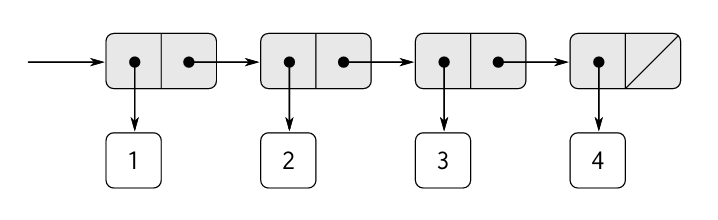
\includegraphics[width=\textwidth]{figures/lisp-list.png}

An empty list is simply the termination symbol and a list of length n is a pair containing an element in one slot and a list of length n - 1 in the other.
Rust's type system understands recursion and provides a singleton unit type along with an ordered pair type - a binary tuple.
Functionality for such lists would need to be expressed using traits since our very goal is to abstract over lists of different types --- so no concrete type could possibly suffice.
With all that in mind, we present a scheme for non--homogenous collections of types in Rust.

Starting with the most basic type list, we define a trait which simply states that given type is a type list (called HLists henceforth \cite{frunk}), and provides no actual functionality.

\begin{lstlisting}
pub trait HList { }
\end{lstlisting}

Then we provide implementations for base and recursive cases.

\begin{lstlisting}
impl HList for () { }
impl<Head, Tail> HList for (Head, Tail) where Tail: HList { }
\end{lstlisting}

We verify that our implementation works with a no--op function that simply checks if passed value is of type that implements \texttt{HList}.

\begin{lstlisting}[basicstyle=\tiny]
fn test<HL>(_: HL) where HL: HList { }

fn main() {
  let list_1: ()                         = ();
  let list_2: (i32, ())                  = (1, list_1.clone());
  let list_3: (f32, (i32, ()))           = (42.0, list_2.clone());
  let list_4: (String, (f32, (i32, ()))) = (String::from("wow"), list_3.clone());

  test(list_1);
  test(list_2);
  test(list_3);
  test(list_4);
}
\end{lstlisting}

Type annotations are redundant, as types can be inferred, and were purposefully added to better visualize the mechanism.
This sample can be run interactively in the rust playground --- an online service hosted by rust foundation that provides 
a browser interface to the Rust compiler to experiment with the language. 
To run this listing follow this \href{https://play.rust-lang.org/?version=stable&mode=debug&edition=2021&gist=0c13e950bb10a01dbae1981b0c15aa5f}{[playground permalink]}.

One can create increasingly complex traits and implement them in a similar manner, for example below we implement HList length computation.

\begin{lstlisting}
pub trait HList { fn len(&self) -> usize; }
impl HList for () {
  fn len(&self) -> usize { 0 }
}
impl<H, T> HList for (H, T) where T: HList {
  fn len(&self) -> usize { self.1.len() + 1 }
}
\end{lstlisting}

\noindent \href{https://play.rust-lang.org/?version=stable&mode=debug&edition=2021&gist=13d2d29f768d207f8fe7fa1bde7acef1}{[playground permalink]}

By deciding in which slot to place the tuple and in which the current element we can change the winding order of the HList.
Both left and right winding schemes are equivalent in terms of functionality, but differ in terms of potential user experience.
In our case appending new types to the end of a HList was by far the most common use case, and as such we almost exclusively use left wound HLists (LHLists)
due to cleaner type signatures being produced that way.

These homogenous collections have been implemented as an independent module called \texttt{hlist} which can be found in the root of our crate.

\paragraph{Use case}

In \texttt{gpu-bulwark} HLists are used every time variable--length user configuration is required, most notably to represent shader inputs, outputs, used uniforms or external resources like textures.
Almost always we create a facade marker trait which joins together predefined pieces of functionality from \texttt{hlist} module
and adds specialized requirements for HList member types in order to prohibit creation of invalid type list.

\subsection{Const generics in const expressions}

\paragraph{Problem}

Const generics fall into the category of partially implemented features. Const generic types depend on a value of limited subset of types, most notably numeric types, bool and unit.
This feature, being in its early stages, has a significant limitation: const parameters must be literals or expressions using only literals. 
Const parameters cannot be used in any type level const expressions, they have to be used directly. 
As a result, we cannot perform arbitrary compile--time computations on these parameters for purposes of verification.

\paragraph{Solution}

However, there is one exception to that limitation: associated constants. Associated constants can have their values computed using compile--time evaluated \texttt{const fn}s and themselves be used in such computations as parameters.
Example with HList length could be adapted to use consts instead of methods like so.

\begin{lstlisting}
pub trait HList { const LENGTH: usize; }
impl HList for () {
    const LENGTH: usize = 0;
}
impl<H, T> HList for (H, T) where T: HList {
    const LENGTH: usize = T::LENGTH + 1;
}
\end{lstlisting}
\noindent \href{https://play.rust-lang.org/?version=stable&mode=debug&edition=2021&gist=05d326a2dc997f8005fb06711fe6fa3f}{[playground permalink]}

These functions can panic with static error message (no formatting) and may cause compilation errors based on programable logic.
Lack of compile--time formatting makes it difficult to provide useful error messages, yet another advantage of using type--based validation.
As a consequence, different limitation was imposed: associated constants cannot be used as const parameters in types, they can only be used as values in code.

\paragraph{Use case}

Due to the lack of negative reasoning, as of yet, in Rust compiler we cannot express type inequality.
As the only viable solution would be tp write a blanket impl stating that two types are different if they are not the same type; since such a blanket would apply to user defined types as well.

CT validation that types are all different is required to assert that glsl variable layout locations do not overlap.
In certain scenarios when layout components are used this overlap may be valid; we ignored it in this work because it can be easily taken into account in future releases.

We use associated constants, conditionally panicking \texttt{const} function and environment variables to allow for compile--time validation that HLists of glsl variables 
of arbitrary length do not overlap.

We prepared an another example in the \href{https://play.rust-lang.org/?version=stable&mode=debug&edition=2021&gist=61baf4a1043d947594ef33d03bb8390b}{playground} where
HLists are checked to contain types with increasing numeric indices assigned to them.

\subsection{Effect system}

\paragraph{Problem}

First class effect system is a non--existent feature that would be of immense value in the context of an OpenGL wrapper implementation.
Ability to type check function invocation context in OpenGL would be especially useful as we could encode presence of appropriate object binding using an effect.

\paragraph{Solution}

We instead were forced to opt for more error prone and verbose approach.
Objects like textures or buffers can produce binder objects which in their constructor bind, and in their destructors unbind, object from the appropriate binding point.
This lets us control context bindings using lexical scope, but does not in any way prevent distinct objects with the same target from overriding the global binding.
A minimal example showing of effect emulation can be found on \href{https://play.rust-lang.org/?version=stable&mode=debug&edition=2021&gist=3724852e646ce5d0ed1faf0c57f3e5c1}{playground}.

\paragraph{Use Case}

As already mentioned above, effect system would greatly improve the handling of context bindings in terms of statically verifiable correctness, as well as, user and developer experience.
Even though in OpenGL 4.6 with direct state access we could circumvent this problem altogether, we purposefully chose to keep it and tried tackling it.

\subsection{Subtyping}

\paragraph{Problem}

Subtyping or inheritance is a very common concept in object oriented programming. 
In these languages, one can create a type and inherit from it to produce more specialized version of the original type -- a subtype.
Subtype extends functionality of base type and can seamlessly delegate all base type's method calls to the base type, and can be used in all places the base type can.

\paragraph{Solution}

Using generic type and automatic dereferencing via \texttt{Deref} we can emulate the relation of subtyping.
The base type has a generic parameter which corresponds to any potential subtype, and implements \texttt{Deref} and \texttt{DerefMut} targeting that subtype.

\begin{lstlisting}
struct Base<Child> { base: i32, child: Child }

impl<Child> Deref for Base<Child> {
    type Target = Child;
    fn deref(&self) -> &Self::Target { &self.child }
}

impl<Child> DerefMut for Base<Child> {
    fn deref_mut(&mut self) -> &mut Self::Target {
        &mut self.child
    }
}

struct Subtype;
type Inherited = Base<Subtype>;
impl Inherited { /* ... */ }
\end{lstlisting}

\noindent \href{https://play.rust-lang.org/?version=stable&mode=debug&edition=2021&gist=8946828515f1f87f388374b6bbc69bca}{[playground permalink]}

Subtype is obtained by defining a type alias for the generic base type with concrete subtype state specified.
Subtype--specific functionality can now be specified using an \texttt{impl} block on this alias.
Such an \texttt{impl} would be coherent since all other subtypes have different nominal types representing their states and have full access to both base type's and subtype's states.

\paragraph{Use Case}

We applied this emulation of inheritance to model OpenGL objects. \texttt{ObjectBase<T>} contains base state and functionality and \texttt{T} provides implementation 
for subtype specific allocation, deallocation and context binding in a scheme very similar to template method pattern.

\section{Validation of program structure at compile--time}

\subsection{Markers}

\paragraph{Problem}

Enumeration types are a core component of almost all currently used programming languages. In recent years, many languages have even gained the ability to store variable--size data in their dynamic enum variants.
Such enums provide simple mechanism for statically typed polymorphism with dynamic variants. 
However, sometimes this dynamic--ness of enums is a hurdle causing constant match or switch statements to pollute the code base, producing clutter and boilerplate.
Sometime one simply wishes to encode static configuration based on a closed set of possible values.

\paragraph{Solution}

Markers are traits and types which don't provide any runtime behavior, but rather exist for purposes of conveying information and constrains on a type level.
Marker traits provide no useful functionality, but rather serve to impose relations and logical division on types.

Marker types don't hold any data and as such don't exist at runtime (they occupy zero bytes and are formally called Zero Sized Types --- ZST).
It is possible for marker types to have type parameters by using special compiler intrinsic datatype \texttt{PhantomData}; which binds parameters, but does not hold any value.

Marker traits along with marker types can be used as:
\begin{itemize}
    \item compile---time enums -- by limiting access to a marker using item visibility qualifiers, we strictly control what types implement given functionality.
    \item marker trait based relations -- we can express relations between types and make unsound parameter combinations a compile--time error.
    \item typing external resources -- by using \texttt{PhantomData} we can attach type information to otherwise untyped parts of an API.
\end{itemize}

\begin{lstlisting}[basicstyle=\tiny]
use std::marker::PhantomData;

/// This pattern of pub trait in private module provides the sealing behaviour.
/// Downstream users cannot use this trait but other public traits can
/// list it in its super traits.
mod sealed {
    /// A marker trait that will be implemented for predefined set of types
    /// from which downstream clients should choose pixel channel types in PixelFormat struct.
    pub trait Channels { }
}

// Four marker types used by pixel format to statically dispatch impl blocks.

pub struct R;
pub struct RG;
pub struct RGB;
pub struct RGBA;

impl sealed::Channels for R { }
impl sealed::Channels for RG { }
impl sealed::Channels for RGB { }
impl sealed::Channels for RGBA { }

/// Using marker types and traits we provide typing information to external resource such as pixels
pub struct PixelFormat<C, const COMPONENT_SIZE: usize>(PhantomData<C>)
where 
    C: sealed::Channels
;

// Now we provide functionality for PixelFormats with channels from predefined
// set of possible configurations.

impl<const N: usize> PixelFormat<R, N> { pub fn r() { println!("R{}", N); } }
impl<const N: usize> PixelFormat<RG, N> { pub fn rg() { println!("RG{}", N); } }
impl<const N: usize> PixelFormat<RGB, N> { pub fn rgb() { println!("RGB{}", N); } }
impl<const N: usize> PixelFormat<RGBA, N> { pub fn rgba() { println!("RGBA{}", N); } }

fn main() {
    PixelFormat::<R, 4>::r();
    PixelFormat::<RG, 8>::rg();
    PixelFormat::<RGB, 16>::rgb();
    PixelFormat::<RGBA, 32>::rgba();
    
    // Error -- we prevent the very creation of nonsensical type.
    // PixelFormat::<i32, 32>;
}
\end{lstlisting}
\noindent \href{https://play.rust-lang.org/?version=stable&mode=debug&edition=2021&gist=7d092a3be5593833894fa27b5fa56757}{[playground permalink]}

\paragraph{Use Case}

We make heavy use of markers to implement entirety of glsl module which consists almost exclusively of ZSTs for purposes of modelling shader \texttt{in}, \texttt{out} and \texttt{uniform} variables.
Types representing these variables aggregated into hlists are specified by the user with help of GLSL DSL implemented using lightweight declarative macros.

Marker traits in miscellaneous \texttt{\_::valid} modules define relations between valid combinations of data types. Buffer in raw OpenGL, 
due to C's lack of generics, has its buffer populated using \texttt{*void} and the documentation enumerates valid types. 
To make things worse validity of data types changes depending on what's the buffer's target.
It is illegal for index buffer to contain anything other than unsigned integers, pixel buffers can contain almost everything, whilst vertex buffers, 
yet again, can contain only specific combinations of data.
By associating a phantom type with a Buffer and using marker trait based validation relations on uploaded data we solve both of these issues.

This methodology can be extended to form \textbf{many modes} pattern, in which one uses marker types that implement trait 
containing generic associated types to control behavior in more complex fashion than using non--generic associated types \cite{nikobloggats}.

\paragraph{many modes}

We use many modes in \texttt{Variable<S, L, T, Store>} to abstract over kind of storage used for variable's type member --- \texttt{Phantom} or \texttt{Inline}.
\texttt{Phantom} uses \texttt{PhantomData} as its associated type and effectively discards value and \texttt{Inline} keeps it as is.

\subsection{Type State}

Type state is a very powerful pattern that takes advantage of how rust understands generic types and allows for tracking runtime capabilities at compile--time.
Its name refers to static verification technique of the same name proposed by Robert E. Strom and Shaula Yemini \cite{typestate}. 
Which allowed to determine the subset of operations permitted on a data object in a particular context,
detecting and preventing semantically undefined execution sequences at compile--time.

This behavior can be elegantly implemented in rust using generics.
For the duration of this subsection it is worth to think about generic types as of type constructors which can be partially applied to create another constructor or fully applied to produce a type.

Recall from the section on coherence \ref{sec:coherence} that Rust determines if \texttt{impl}s are non--overlapping, what it implies is that each associated item can be resolved uniquely.
Additionally \texttt{impl} blocks can be generic and implemented for generic types. These \texttt{impl}s can be generic over a subset of parameters, 
by providing fixed types for certain parameters.

\begin{lstlisting}
struct Generic<T, H, F>(T, H, F);

impl<F, H> Generic<i32, F, H> { /* ... */ }
impl<F, H> Generic<u32, F, H> { /* ... */ }
impl<H> Generic<u32, (), H> { /* ... */ }
\end{lstlisting}

Rust understands that \texttt{Generic<i32, F, H>} and \texttt{Generic<u32, F, H>} must be different types (note the difference \texttt{i32} and \texttt{u32}),
and as such any implementations for these two types must be disjoint.
This behavior is what empowers type state pattern. We can intentionally add or use an existing generic parameter (const parameters can be used as well)
to encode certain states and provide functionality for the main type in that specific state. Along with state specific type capabilities state transitions between the states are provided,
allowing to encode a compile--time state machine.

In the below listings we show how type state, along with markers could be used to statically guarantee, that only users who were successfully authenticated
can access secret information. We start by creating marker types \texttt{Anonymous} and \texttt{Verified} which represent different states a user session can be in.
We constrain the possible set of state types, and assign each state its own data with \texttt{AuthenticationStatus}.

\begin{lstlisting}
pub trait AuthenticationStatus {
    type Ctx: Sized;
}

pub struct Verified;
pub struct Anonymous;

/// Empty state is associated with an anonymous user.
impl AuthenticationStatus for Anonymous {
    type Ctx = ();
}

/// Representation of a user.
pub struct User {
    pub user_name: String,
    /* ... */
}

/// If user is logged in, User data can be obtained.
impl AuthenticationStatus for Verified {
    type Ctx = User;
}
\end{lstlisting}

To represent a permanent connection (like a TCP socket) we created the \texttt{Connection} type.
Its a simple wrapper around IPv4 socket address thats used solely as a identifier, no actual network connections are made.
Its purpose it to demonstrate that type state can accommodate persistent data by moving it between states.

\begin{lstlisting}
struct Connection(Ipv4Addr);

impl Connection {
    pub fn new(client: Ipv4Addr) -> Self {
        println!("connection established with: {:?}", &client);
        Self(client)
    }
}

impl Drop for Connection {
    fn drop(&mut self) {
        println!("connection closed with: {:?}", &self.0);
    }
}
\end{lstlisting}

Finally we define type state based \texttt{Session} type.

\begin{lstlisting}
struct Session<AS> where AS: AuthenticationStatus {
    type_state: PhantomData<AS>,
    connection: Connection,
    ctx: AS::Ctx,
}

impl Session<Anonymous> {
    fn new(ip: Ipv4Addr) -> Self {
        Self {
            type_state: PhantomData,
            connection: Connection::new(ip),
            ctx: (),
        }
    }
}

impl Session<Verified> {
    fn secret(&self) -> String {
        "'a secret'".into()
    }
}
\end{lstlisting}

Session in each state holds a \texttt{Connection} instance, phantom data and ctx to store current state type and any data associated with it.
We then precede to define semantics of our type state. 
We allow direct creation of only anonymous sessions, and for access to secret information for authenticated sessions. 
Now all that remains are the state transitions.

\begin{lstlisting}
#[derive(Error, Debug)]
enum LoginError {
    #[error("invalid password for {user_name}: {password}")]
    InvalidPassword { user_name: String, password: String },
}

fn db_check_password(user: &User, password: &str) -> Result<(), LoginError> {
    (password == "password")
        .then_some(())
        .ok_or(LoginError::InvalidPassword {
            user_name: user.user_name.clone(),
            password: password.into(),
        })
}

impl Session<Anonymous> {
    /// We provide ability to log in only for anonymous users.
    pub fn log_in(self, user: User, password: &str) -> Result<Session<Verified>, LoginError> {
        db_check_password(&user, password).map(|_| Session {
            type_state: PhantomData,
            connection: self.connection,
            ctx: user,
        })
    }
}
\end{lstlisting}

We provide some basic mocks of the authentication mechanism and use it to define the \texttt{log\_in} method on \texttt{Session<Anonymous>}.
It consumes an anonymous session, validates given credentials and constructs validated session's instance if validation was successful,
which is the only way to obtain an instance of the \texttt{Session<Verified>} type.
That's how type state enforces that only logged in users can access secret information. This invariant is guaranteed at compile-time.
However, if the actual transition succeeds is determined at runtime. We statically enforced a sequence of operations, and prevented
function invocation sequence which is semantically incorrect.

A full sample along with few examples can be accessed via \noindent \href{https://play.rust-lang.org/?version=stable&mode=debug&edition=2021&gist=bb0ff57d61dcdc9f4473cf51bec012a3}{[playground permalink]}.

\section{OpenGL wrapper}
  
\subsection*{Scope}

Our goal with this study was foremost to explore how Rust's type system can be utilized to improve static validation of OpenGL programs.
We by no means meant to cover the entirety of OpenGL functionality, only the most essential aspects like shaders, programs, vertex arrays and buffers and textures.
Nevertheless, a great deal of consideration was taken before every major design decision to ensure that one could simply duplicate existing solution from a single 
API variant to all others and obtain the same level of functionality and protection.
Additionally, we tried staying as true to original OpenGL API as possible. We preserves most of the semantics, function names and parameters that made sense.
All objects don't retain any parameters, they simply forward them to appropriate GL procedure calls. 

In the end we arrived at minimal working example of a type--driven OpenGL 4.6 core wrapper that provides ability to create all the aforementioned GL objects,
and program even moderately complex computer graphics applications in a safer fashion.

\subsection{GLSL module}

Programming in OpenGL consists of GL API and GLSL shaders. This division is at very core of our library as it's essential to correctly capture how glsl and opengl interact.

We settled on a design were shaders and pipeline configuration are the original source of truth and that's were \texttt{gpu-bulwark}'s user must start development.
Description of graphics pipeline and everything related to glsl is encompassed in the \texttt{glsl} module.
The most important component of that module is the \texttt{Variable<S, L, T, Store = md::Phantom>} type.
It represents an AST--like node for glsl variable at a type level.
It contains type parameters for 3 qualifiers we discussed in chapter 2: Type, Storage and Layout. These qualifiers are most essential from the perspective of correctness verification.
We use the \texttt{Variable}'s type parameters as follows:
\begin{itemize}
    \item type qualifier --- it is used most notably in matching vertex array's attribute definitions and shader matching during program construction.
    \item storage qualifier --- since variables with different storage qualifiers can share the same locations its imperative to distinguish between storage qualifiers during location overlap checking.
    \item layout qualifier --- both location and binding values are used along with previous qualifiers to determine if shader inputs, outputs or uniforms are defined in a valid way.
\end{itemize}

Additionally \texttt{glsl} defines compatibility between glsl \texttt{in} types and gl attribute types.

\subsection{Shaders}

\texttt{gpu-bulwark} provides type state builders for complex objects like shaders or programs. Type state builder has a state for each type parameter we determined that object requires.
In case of shader it has one state parameter that corresponds to compilation status. The \texttt{create} method creates a shader in \texttt{Uncompiled} state.

In this state the only operation one can perform is provide shader source code. In order to attach a shader to a program, shader needs to be compiled. 
Compilation can either succeed and return shader object now in \texttt{Compiled} state or a compilation error back to the user.
Once shader has been compiled successfully one can specify what uniform variable this shader requires or precede forward by converting shader 
to either shader containing a pipeline stage entry point \texttt{main}, or to \texttt{Lib} shader for use for linking.
\texttt{Main} shader require specification of inputs or outputs using appropriate \texttt{glsl::Variable}s.

Such shaders are ready for attachment to program Objects.

\subsection{Program}

In this study we implement non--separable program objects, which means that at least vertex and fragment shaders need to be specified, as well as, that all stages have to match during linking.

\subsubsection{Builder}

Program is built using the most complex type state builder. It contains six type parameters corresponding to
\begin{itemize}
    \item target shader of most recently attached shader with entrypoint
    \item vertex input
    \item outputs of most recently configured stage
    \item program uniform definitions
    \item uniform declarations from most recently configured stage
    \item declarations of external resources used by the program
\end{itemize}

Program building is divided into two parts: (1) uniform specification and (2) pipeline configuration.


\subsubsection{Uniform Specification}

During uniform specification one can define uniforms that program contains by defining their type and providing their initial values, along with declarations of external resources that program uses.
Although both are represented by uniforms in GLSL transparent uniforms differ in their meaning from opaque types which all represent handles to resources external to the program
instead of plain old data like matrices or vectors.

\subsubsection{Pipeline Configuration}

Once uniforms and resource declarations and configures, builder transitions to vertex shader stage where obligatory main entrypoint for vertex stage needs to be provided.
From here type state will force the user to follow valid configuration paths for the pipeline as defined in the specification, 
validating that outputs from most recently attached entrypoint shader match inputs to the newly provided one using location layout qualifiers 
on shader provided inputs and outputs, resulting in compilation error in case of a mismatch. 
This traversal always concludes with specification of the fragment stage entrypoint, after which linking can be performed and actual Program object obtained.

If program is obtained it means that pipeline is configured correctly, program is linked and ready for use. Otherwise either compilation or runtime program link error was generated.
In the current version we do not validate that representation of shader interfaces actually matches shader status, but it can be easily achieved 
by either parsing shader source code or querying shaders interfaces using OpenGL introspection API.

\subsection{Buffer}

Buffer objects heavily leverage phantom types and markers to provide type information and content validation, to what otherwise would be a basic integer resource descriptor.

Buffers are created, as for all objects, with \texttt{create} function.
Once buffer is created its data store can be allocated and populated with \texttt{data} function which expects one type parameter for usage hint.

\subsection{Memory Mapping}

Buffers have an interesting feature that they can be mapped into memory and used with Direct Memory Access.
We provide this functionality using auxiliary \texttt{Mapped\_} types which borrow a buffer and are smart pointers that provide \texttt{Deref} and \texttt{DerefMut} to slices,
allowing for idiomatic store access.
A noteworthy implementation detail is that \texttt{Mapped\_} smart pointers, leverage the borrow checker to safeguard against an error condition during rendering
where draw call was issues using vertex array that sources vertex data from memory mapped buffer. 
Smart pointers hold references to buffers borrowed in turn from VAO, and since \texttt{draw\_arrays} method also requires mutable reference to VAO borrow checker will reject
a program if any buffer used as vertex source is mapped during drawing.

\subsection{Vertex Array}

Vertex Array can be created with \texttt{create}. It exposes a single method \texttt{vertex\_attrib\_pointer} which takes ownership of a Buffer bound to \texttt{BUFFER\_ARRAY}
and an \texttt{in} variable to associate given buffer with as an \texttt{Attribute}.
Attributes encompass buffer, vertex format and attribute index. This is a complete set of information needed to match vertex shader input variables.
and stores it in VAOs internal HList of \texttt{Attribute}s. 
Buffer object must contain data which is deemed \texttt{Compatible} with program's input at a matching location.
Compatibility is determined based on implementation of our internal unsafe trait \texttt{ffi::FFI} which states that for any non glsl type, bytes of type implementing it,
can be safely reinterpreted as array of given type and size. 
We implemented this traits for arrays, scalars and even integrated it with \texttt{nalgebra} crates,
as well as for phantom types from the \texttt{glsl} module.
During buffer content matching we check, that type which it contains, has the same ffi layout as corresponding glsl variable expects, using equality bound on types as discussed in \ref{sec:assoctypes}.
This allows us to provide data for \texttt{mat2} using \texttt{[f32; 4]}, \texttt{[[f32; 2]; 2]} or \texttt{nalgebra::Matrix2}.

\subsubsection{Draw Calls}

There are three variants of regular \texttt{draw\_arrays}. First is designed for programs with no inputs, outputs, uniforms and resources --- ones which essentially have the entire scene
encoded in shader sources code. 
Second expects vertex array object which it binds and draws as many triangles as VAO specifies. Types of attributes are checked for compatibility against program inputs defined using glsl variables.
Finally the third version, the most general, expects VAO and handles to texture bindings which are matched against external resources program uses. 

\subsection{Textures}

Textures have the broadest API of all the OpenGL objects.
Textures consist of three components: (1) sampling parameters, (2) texture parameters and (3) texture images, but only the storage benefits 
from strong typing due somewhat complex allocation and wide range of rules regarding valid parameter combinations which all can be easily expressed and checked at compile--time.

Textures support mipmaps in order better antialias textures during sampling. 
Mipmaps are a sequence of images generated from original image by halving its dimensions until they all reach 1px.
For a well defined behavior all mipmap levels must be allocated in the correct way, this requirement is called texture's mipmap completeness.

\subsubsection{Storage}

When texture is created its storage kind (immutable, mutable, buffer) and textures dimensionality (1D, 2D or 3D) are defined by the function name.

Textures can have 3 types of their storage
\begin{itemize}
    \item mutable texture owned --- allocated using \texttt{TexImage*} family of functions. 
        This was historically the earliest form of texture storage, and thus suffers the most from issues related to backwards compatibility. 
        This kind of storage can be later reallocated, hence mutability. 
        Mipmaps need to be manually allocated and uploaded which is quite error prone, 
        since if texture is not mipmap complete using it causes undefined behavior.
        Pixel data for mutable storage can be specified directly using
        \texttt{TexImage*} \texttt{data} parameter or a Buffer bound to \texttt{PIXEL\_UNPACK\_BUFFER}.
        Data may also be modified using \texttt{TexSubImage*} functions.
    \item immutable texture owned --- allocated using \texttt{TexStorage*} family of functions. 
        This is the most recently added kind of texture backing storage. 
        Once texture with this storage is allocated it cannot be reallocated. 
        Major benefit of using immutable textures is that mipmaps are allocated automatically. 
        Storage immutability allows to create views into the texture providing 
        an opportunity for better memory conservation, and substantially simplifies work for the driver.
        Pixel data for these kinds of storage must be supplied using \texttt{TexSubImage*} functions.
    \item buffer backed texture --- memory and content of texture come from buffer bound to \texttt{BUFFER\_TEXTURE},
        and similarly such a texture must be also bound to \texttt{BUFFER\_TEXTURE}.
\end{itemize}

In our work we focussed on immutable storage textures due to their automatic mipmap allocation which frees us from 
implements compile--time mipmap completeness validation.

\subsubsection{Image Format}

Image formats (texture's internal format) are implemented in \texttt{texture::image} module.
They describe memory layout pixels in GPU's memory and their interpretation.
We focused on implementing sized formats as they specify precisely component count and size 
and such precision lends itself well to type level validation.
They are represented by a \texttt{Format<Components, ComponentType, Interpretation>}.
Besides component count and type, image formats have one additional parameter: \texttt{Interpretation},
it symbolizes how shader should interpret these values: either integers or floats.

\subsubsection{Pixels}

Once texture is allocated it needs to be initialized with pixels, by means of a pixel transfer operation.
The simplest way to transfer pixel data is by using \texttt{TexSubImage*} functions.
Ranges along each texture dimension have to be specified where pixels will be substituted,
along with pixel's type and format.
These to parameters are expressed using traits and implemented for Rust's arrays of appropriate size and content.
Format parameter has dual meaning it describes: (1) what texture channels to target with current pixel transfer
(which indirectly determines number of components in provided data) with formats like \texttt{RED}, \texttt{GREEN}, \texttt{BLUE},
\texttt{BGRA} or \texttt{BGR}, and how pixels are to be interpreted during texture sampling --- as integers or floats --- which needs to match
texture's image format \texttt{Interpretation} parameter.

Pixel transfer operations are implemented in such a way that type inference treats internal format's types
as valid ones and will validate pixels that user is trying to transfer against that and report a compilation error
if pixels are not compatible.

\section{Examples}

Examples demonstrating usage of \texttt{gpu-bulwark} are provided in \texttt{examples} directory, located in the root of the project.
There are four samples which increase in complexity as follows:
\begin{itemize}
    \item \texttt{hello\_triangle} --- the simplest example that shows the most basic rendering scenario where program is hard coded to produce a white
        triangle on the screen
    \item \texttt{hello\_vertices} --- this sample demonstrates basic vertex attribute configuration using a vertex buffers, 
        vertex array and program input and VAO attribute matching. 
        Two vertex attributes are used: one for vertex positions and another for vertex color.
        This sample is interactive, user can use A, S and D keys to modify color values stored in buffers 
        which is implemented using buffer memory mapping and using buffers via normal rust slices.
    \item \texttt{hello\_textures} --- example of how to use textures. By pressing A, S, D user can change the displayed bitmap.
    \item \texttt{hello\_uniforms} --- sample that shows how more complex programs which use uniforms may be constructed.
        Program implements an interactive 3D camera which can be controlled with mouse and keyboard to navigate in 3D space and
        view the scene: a single rainbow triangle which can be shrunk using space bar. This interactivity is produced by using two uniform variables: 
        (1) view--perspective matrix and (2) a float uniform that scales the triangle. Sample can be closed with the escape key.
\end{itemize}
